\documentclass[10pt,a4paper]{article}
\usepackage[utf8]{inputenc}
\usepackage[T1]{fontenc}
\usepackage{lmodern}
\usepackage[a4paper,margin=2.2cm]{geometry}
\usepackage{graphicx,booktabs,amsmath,amssymb,array,float}
\usepackage[hidelinks]{hyperref}
\usepackage[font=small,labelfont=bf]{caption}
\usepackage{microtype}
\usepackage{titlesec}
\titleformat{\section}{\large\bfseries}{\thesection.}{0.5em}{}
\titleformat{\subsection}{\normalsize\bfseries}{\thesubsection}{0.5em}{}
\titlespacing*{\section}{0pt}{10pt}{4pt}
\titlespacing*{\subsection}{0pt}{6pt}{2pt}
\setlength{\parskip}{3pt}
\setlength{\parindent}{0pt}
\graphicspath{{../results/figures/}{./}}

\begin{document}

\begin{center}
{\LARGE\bfseries Interval Type-2 Fuzzy Green-Time Control of a Signalised Intersection:\\[2pt]
Re-implementation, Optimiser Comparison and Detector-Noise Robustness}\\[8pt]
{\large Fuzzy Logic Course -- Term Project Report}\\[4pt]
\textbf{Student:} [Full name]\quad \textbf{Student no.:} [number]\quad \textbf{Date:} November 2026\\[2pt]
\textbf{Reference paper:} E.~Korkmaz and A.~P.~Akg{\"u}ng{\"o}r, \emph{Soft Computing} 28:7227--7249, 2024 \cite{ref_paper}\\[2pt]
\textbf{Code:} \texttt{github.com/[user]/fuzzy-logic-project} (repository link to be filled in)
\end{center}

\begin{abstract}
Korkmaz and Akg{\"u}ng{\"o}r \cite{ref_paper} propose a hybrid traffic signal controller in which an interval Type-2 Sugeno fuzzy system, tuned by the crow search algorithm (CSA), adjusts the next green time by $\pm6$~s. Because the authors' simulator and code are not public, we re-implement the fuzzy green-time part in our own event-based intersection simulator and repeat the paper's main experiment on 18 demand scenarios (3 and 4 legs, 20 seeds). Tuned Type-1 and Type-2 controllers reduce delay by about 10\% against well-set fixed-time control, but the extra benefit of Type-2 over Type-1 reported in the paper is not reproduced ($-0.1$\% and $-0.5$\%). As extensions we compare four optimisers at equal budget (CSA equals DE and beats FPA and PSO), test robustness to detector noise up to 75\% (IT2 degrades slightly less, not significantly), compare Karnik--Mendel with Nie--Tan type reduction (0.6\% more delay for one-third cheaper inference) and show that longer tuning over-fits. All code, data generation and results are reproducible from the repository.

\end{abstract}

\section{Introduction}
Delays at signalised intersections are a major component of urban travel time, and a fixed-time plan cannot follow the random
fluctuation of arrivals. Fuzzy logic is a natural tool here: ``few'', ``many'', ``short queue'' and ``long queue'' are linguistic
statements that traffic engineers already use, and a rule base can turn them into a green-time decision without an analytical model of
the traffic stream. Korkmaz and Ak{\"g}{\"u}ng{\"o}r \cite{ref_paper} combine this idea with two metaheuristics: the flower pollination
algorithm (FPA) selects the phase plan and cycle length, and an interval Type-2 Sugeno fuzzy system whose membership functions (MFs)
are tuned by the crow search algorithm (CSA) lengthens or shortens the next green by up to $\pm 6$~s. The resulting hybrid controller (HTSC)
is reported to reduce delay by about 32\% against fixed-time control and by 5--6\% against an FPA-only controller and a Type-1 fuzzy controller.

\textbf{Goal of this project.} The reference code and the simulator (KU-Trsim) are not public. The project therefore (i) re-implements the fuzzy
green-time part of the method from the paper description, in a simulator written for this study, (ii) re-runs the paper's main
experiment (nine demand scenarios, 20 random seeds, fixed-time versus FPA versus Type-1 versus Type-2 control), and (iii) adds three
controlled extensions that the paper does not contain: a comparison of four optimisers for the Type-2 MFs, a detector-noise robustness
study, and a comparison of type-reduction methods together with computational cost.

\textbf{Summary of findings.} Tuned fuzzy controllers reduce delay by about 10\% against fixed-time control, which is of the same order as the
paper's Type-1 result for three legs (8.6\%) but lower than for four legs (19.8\%). The additional benefit of interval Type-2 over Type-1 reported by the paper was \emph{not} reproduced in our
setting (Section~\ref{sec:results}). The report states which differences between our set-up and the paper may explain this, and every number in the
tables is produced by the code in the accompanying repository.

\section{Related Work}
Fuzzy traffic signal control has been studied for more than two decades; surveys are given in \cite{koukol2015,agrahari2024}.
Table~\ref{tab:related} lists the studies most closely related to the reference paper, with results as they are summarised in the
introduction of \cite{ref_paper} (these figures come from different simulators and baselines and are not directly comparable).
Early controllers used Type-1 fuzzy sets, either to extend the current green \cite{trabia1999} or with MFs and rules tuned by
particle swarm optimisation \cite{chen2006} or differential evolution (DE) \cite{dogan2016}. Type-2 controllers followed because traffic
data are noisy: Balaji and Srinivasan \cite{balaji2009} used a multi-agent Type-2 architecture, Bi \emph{et al.} \cite{bi2014} tuned
Type-2 MFs and rules with DE, Araghi \emph{et al.} \cite{araghi2017} compared cuckoo search, GA and simulated annealing for an
interval Type-2 ANFIS controller, and Khooban \emph{et al.} \cite{khooban2017} optimised a general Type-2 controller with a modified
backtracking search. The same authors as the reference paper showed earlier that FPA alone can optimise phase plan, sequence and green
times \cite{korkmaz2021a}. More recent work combines fuzzy systems with learning: Bi \emph{et al.} \cite{bi2024} let a Type-2 fuzzy
controller set the phase green time inside a Deep Q-Network on a single intersection (SUMO simulation), and the 2022 studies cited in \cite{ref_paper}
use fuzzy control with DE \cite{lin2022}, CNN-LSTM \cite{islam2022} or reinforcement learning \cite{zhao2022}. The review \cite{agrahari2024}
notes that more work is needed beyond the single-intersection setting.

\begin{table}[t]
\centering\small
\caption{Closely related studies (results as summarised in \cite{ref_paper}, except the last row).}\label{tab:related}
\begin{tabular}{@{}p{3.2cm}p{2.7cm}p{2.1cm}p{5.6cm}@{}}
\toprule
Study & Fuzzy type & Optimiser & Reported effect \\ \midrule
Trabia \emph{et al.} 1999 \cite{trabia1999} & Type-1, two-stage & -- & 9.5\% less delay than actuated control \\
Chen \& Xu 2006 \cite{chen2006} & Type-1 (MFs+rules) & PSO & large delay reduction under time-varying demand \\
Balaji \& Srinivasan 2009 \cite{balaji2009} & Type-2, multi-agent & -- & about 66\% less delay (Singapore data) \\
Bi \emph{et al.} 2014 \cite{bi2014} & Type-2 (MFs+rules) & DE & less delay/queue/stops than Type-1 and fixed \\
Do{\u g}an \& Ak{\"g}{\"u}ng{\"o}r 2016 \cite{dogan2016} & Type-1 & DE & 52/48/14\% (low/medium/high demand) \\
Araghi \emph{et al.} 2017 \cite{araghi2017} & interval Type-2 ANFIS & CS, GA, SA & 31/17/3\% vs fixed time \\
Khooban \emph{et al.} 2017 \cite{khooban2017} & general Type-2 & MBSA & less queue and delay than Type-1 and fixed \\
Korkmaz \& Ak{\"g}{\"u}ng{\"o}r 2021 \cite{korkmaz2021a} & -- (phase/green) & FPA & 12--30\% vs fixed, 0.8--3\% vs fuzzy \\
Korkmaz \& Ak{\"g}{\"u}ng{\"o}r 2024 \cite{ref_paper} & interval Type-2 Sugeno & FPA + CSA & about 32\% vs fixed, 5--6\% vs FPA/Type-1 \\
Bi \emph{et al.} 2024 \cite{bi2024} & Type-2 + DQN & DQN & improved flow in SUMO (no figure checked) \\ \bottomrule
\end{tabular}
\end{table}

\textbf{Gap addressed here.} The papers above tune Type-2 controllers with one metaheuristic at a time and mostly report noise-free
simulation. It is therefore not clear (a) whether CSA is a good choice compared with FPA, PSO and DE under an \emph{equal} evaluation budget,
and (b) whether the footprint of uncertainty of a Type-2 system actually buys robustness against detector errors, which is the main argument
for Type-2 in traffic control. These two questions are the proposed extension of this project.

\section{Theoretical Background}
\subsection{Fuzzy sets, linguistic variables and Sugeno inference}
A fuzzy set $A$ on a universe $X$ is described by a membership function $\mu_A: X\to[0,1]$ \cite{zadeh1965}; a linguistic variable
takes values such as \emph{low}, \emph{normal}, \emph{high} that are each modelled by such a set \cite{zadeh1975}. In this work every
input uses triangular MFs $\mu(x)=\max\{0,\min[(x-c+w_l)/w_l,\;(c+w_r-x)/w_r]\}$ with apex $c$ and legs $w_l,w_r$. A zero-order Sugeno system
\cite{takagi1985} has rules ``IF $x_1$ is $A_i$ AND $x_2$ is $B_j$ THEN $y=z_{ij}$'' with crisp consequents. With the minimum t-norm,
the firing strength is $w_{ij}=\min\{\mu_{A_i}(x_1),\mu_{B_j}(x_2)\}$ and the output is the weighted average
\begin{equation}\label{eq:sugeno}
y=\frac{\sum_{r} w_r z_r}{\sum_{r} w_r}.
\end{equation}
Fuzzification, rule evaluation and this weighted average (which replaces a separate defuzzification stage in Sugeno systems) are the
three stages of the Type-1 controller.

\subsection{Interval Type-2 fuzzy logic}
An interval Type-2 set is bounded by an upper MF $\bar\mu_A$ and a lower MF $\underline\mu_A$; the region between them is the
footprint of uncertainty (FOU) \cite{liang2000,mendel2017}. The rule firing strength is now an interval
$[\underline w_r,\bar w_r]$ obtained by applying the t-norm to the lower and to the upper memberships. The output of a Sugeno IT2 system is
an interval $[y_l,y_r]$,
\begin{equation}\label{eq:km}
y_l=\min_{k}\frac{\sum_{i\le k}\bar w_i z_i+\sum_{i>k}\underline w_i z_i}{\sum_{i\le k}\bar w_i+\sum_{i>k}\underline w_i},\qquad
y_r=\max_{k}\frac{\sum_{i\le k}\underline w_i z_i+\sum_{i>k}\bar w_i z_i}{\sum_{i\le k}\underline w_i+\sum_{i>k}\bar w_i},
\end{equation}
with the consequents sorted $z_1\le\dots\le z_R$. The iterative Karnik--Mendel (KM) procedure \cite{karnik2001} finds exactly these
optimum switch points; here Eq.~\eqref{eq:km} is evaluated directly with prefix sums, which gives the same result and was checked
against brute-force enumeration (\texttt{tests/test\_fuzzy.py}). The crisp output is $y=(y_l+y_r)/2$. The Nie--Tan method \cite{li2018nt}
is a closed-form alternative, $y=\sum_i \tfrac12(\underline w_i+\bar w_i) z_i/\sum_i\tfrac12(\underline w_i+\bar w_i)$. When the FOU vanishes, the system
reduces to the Type-1 system of Eq.~\eqref{eq:sugeno} (also tested).

\subsection{Metaheuristics used}
All four optimisers search the unit cube $[0,1]^D$ of encoded MF parameters and minimise the mean delay.
\textbf{CSA} \cite{askarzadeh2016}: crow $i$ follows a random crow $j$ towards its memory $m_j$,
$x_i\leftarrow x_i+r_i\,fl\,(m_j-x_i)$ if $r_j\ge AP$, otherwise it moves to a random position; the memory is updated if the new position is better
($AP=0.05$, $fl=2$ as in the reference paper). \textbf{FPA} \cite{yang2012}: with probability $p$ a global step
$x_i\leftarrow x_i+\gamma L(\lambda)(g^*-x_i)$ with L\'evy-distributed step $L$ (Mantegna's algorithm \cite{mantegna1994}), otherwise a local step
$x_i\leftarrow x_i+\epsilon(x_j-x_k)$ ($p=0.8$, $\lambda=1.5$, $\gamma=0.1$). \textbf{PSO} \cite{kennedy1995} (constriction-type
weights $w=0.7298$, $c_1=c_2=1.49618$) and \textbf{DE} \cite{storn1997} (rand/1/bin, $F=0.5$, $CR=0.9$) serve as widely used references.

\subsection{Delay models}
Webster's method \cite{webster1958} gives the cycle $C_0=(1.5L+5)/(1-Y)$ and green splits proportional to the critical flow ratios.
The HCM control delay used as the FPA objective is $d=d_1\,PF+d_2+d_3$ with uniform delay $d_1=0.5C(1-g/C)^2/[1-\min(1,X)\,g/C]$ and incremental
delay $d_2=900T[(X-1)+\sqrt{(X-1)^2+8kIX/(cT)}]$ \cite{hcm2000}.

\section{Original Method}
\label{sec:original}
The hybrid traffic signal controller (HTSC) of \cite{ref_paper} controls one isolated intersection and consists of four modules
(Fig.~\ref{fig:arch}).

\begin{figure}[t]
\centering
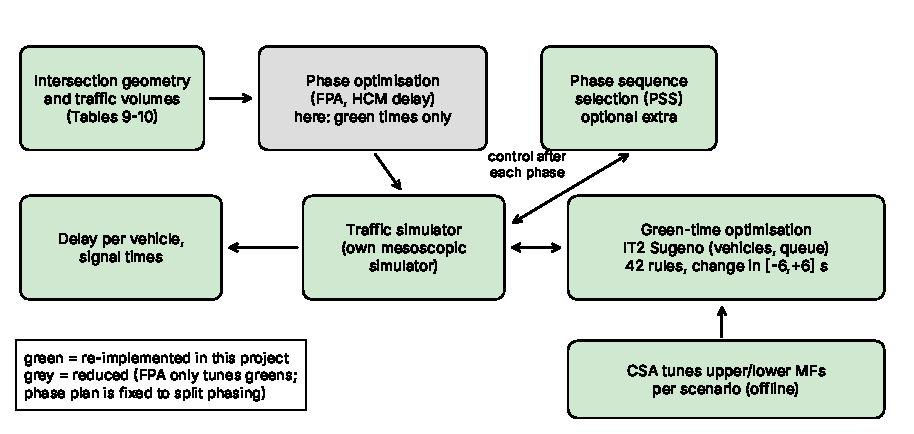
\includegraphics[width=0.92\linewidth]{fig_architecture.pdf}
\caption{Architecture of the reference HTSC (left) and the parts re-implemented in this project (grey box: reduced to FPA green-time tuning with a fixed split-phase plan).}\label{fig:arch}
\end{figure}

\textbf{Phase optimisation (FPA).} For a given geometry and demand, FPA searches the green times of all candidate phase plans (2, 3 or 4 phases),
using the flow-weighted HCM delay as objective, with $8\le g_i\le 60$~s, a degree-of-saturation limit $X\le1.4$, and a safety rule that allows a
permitted left turn only if (left-turn volume) $\times$ (conflicting volume) $<50\,000$. The plan with the lowest delay and its cycle length are kept;
the module is re-run every three cycles.

\textbf{Signal timing optimisation (interval Type-2 Sugeno).} At the end of every phase the controller reads two detector values for the
\emph{next} phase and returns a green-time change in $[-6,+6]$~s. The inputs are the number of vehicles in the 175~m detector range
(universe 0--40, 7 MFs) and the queue length (universe 0--175~m, 6 MFs); this gives $7\times6=42$ rules. The output has seven singletons
($-6,-4,\dots,+6$~s, Table~8 of the paper). The $\pm6$~s interval was selected by trying $\pm4$, $\pm6$, $\pm8$ and $\pm10$~s and an ANOVA
(Tables~6--7 of the paper). The centres and legs of the upper and lower triangular MFs are tuned by CSA, separately for each traffic scenario, with the
objective of minimum delay (Table~5 of the paper).

\textbf{Phase sequence selection.} Among the phases not yet served in the cycle, the one with most vehicles is served first.

\textbf{Experiments.} The system is evaluated in the authors' simulator KU-Trsim (exponential arrivals, Greenshields speed--density relation,
five vehicle types, 900~s runs) on four geometries (3-leg and 4-leg, each with and without left-turn pocket) and nine demand scenarios
(Tables~9--10), averaging 20 random seeds. Competitors are a fixed-time controller, FPA-TSC (phase optimisation only) and a Type-1 fuzzy controller
tuned with DE \cite{dogan2016}. Performance is the mean delay per vehicle, compared with the mean percentage error (MPE, Eq.~11 of the paper) and a Friedman test.
Reported improvements of HTSC over fixed time range from 11.6\% (3-leg) to 31.5\% (3-leg with pocket) (Table~13 of the paper).

\subsection*{Critical reading of the paper}
The following points were noted while reading and are taken into account in this study.
\begin{itemize}\setlength\itemsep{0pt}
\item The rule table, the height of the lower MFs, the population size of CSA and the training/evaluation seed policy are not stated, so exact replication is impossible. It is not stated whether the MFs were tuned and evaluated on the same simulation seeds, which would favour the tuned system.
\item The abstract's ``about 32\%'' improvement equals the best case in Table~13; the mean over the four geometries is lower (about 23.5\% when the four HTSC-versus-fixed entries are averaged). The ``approximately 60\%'' in the conclusions is derived from Friedman ranks, which are not percentages of delay.
\item Eq.~11 as printed gives positive values for an improvement, whereas Table~13 prints negative values; the caption of Fig.~16 says ``three-leg'' for a four-leg figure.
\item Table~7 does not label whether 0.992 is the Levene statistic or its $p$-value, and the ANOVA on $\pm4\dots\pm10$ pools six very different scenarios per group, so a non-significant $F$ cannot be read as equality of the intervals.
\item The Friedman test uses the nine scenarios per geometry as blocks; these are not independent random samples, so the $p$-values describe these nine cases only.
\item The advantage of Type-2 over Type-1 comes from a comparison in which the two systems differ in structure, optimiser (CSA versus DE) and phase optimisation, so the contribution of Type-2 alone is not isolated.
\item High demand saturates the intersection and all controllers approach fixed time; computing time of the optimisers is discussed qualitatively but not measured.
\end{itemize}

\section{Reproduction Methodology}
\label{sec:repro}
Because the reference simulator and code are unavailable, the minimum reproduction requirement (MRR) fixed for this project is the
\textbf{Type-1 and interval Type-2 Sugeno green-time controller with CSA-tuned MFs, evaluated on the 18 demand scenarios of the 3-leg and 4-leg geometries}, compared with
fixed-time and FPA-optimised fixed-time control. All code was written for this project with the help of an AI assistant (see the Generative AI Usage Disclosure); no code of the authors was used. Table~\ref{tab:diff} lists how the
re-implementation differs from the paper; these differences are the main reason why absolute delays cannot be compared with the paper.

\begin{table}[t]
\centering\small
\caption{Differences between the reference study and this re-implementation.}\label{tab:diff}
\begin{tabular}{@{}p{3.2cm}p{5.4cm}p{5.6cm}@{}}
\toprule
Aspect & Reference paper & This project \\ \midrule
Simulator & KU-Trsim, microscopic, acceleration tables & event-based mesoscopic, saturation headway $2.0\times$ vehicle factor (assumed) \\
Phase plan & FPA chooses 2/3/4-phase plan & split phasing (one phase per leg); FPA only tunes greens \\
Geometries & 3-leg, 4-leg, each $\pm$ left-turn pocket & 3-leg and 4-leg (no pocket variants) \\
Rule table & not published & monotone table of 42 rules (own design, Eq.~\eqref{eq:rule}) \\
Lower MF & read from figures & same apex, narrower legs, height 0.5 (assumed) \\
CSA budget & 2000 iterations, population not stated & 20 crows $\times$ 100 iterations, tuned on 4 seeds \\
Evaluation & 20 seeds (tuning seeds not stated) & 20 \emph{different} seeds, common random numbers \\
Type-1 baseline & DE-tuned FL \cite{dogan2016} & same structure and same CSA tuning as the Type-2 system \\
Phase sequence & used in HTSC & optional (reported as an extra row) \\ \bottomrule
\end{tabular}
\end{table}

\textbf{Simulator.} Vehicles of five types (80/10/5/3/2\%, lengths from Table~2 of the paper) arrive with exponential headways, are assigned to one of two lanes
and traverse the 175~m detector range at 50~km/h. A queue discharges with start-up lost time 3.6~s and a headway of 2.0~s multiplied by a vehicle factor
(1.0/1.15/1.8/2.0/1.6 for car/minibus/bus/lorry/truck, assumed because the Synchro acceleration tables are not reproduced); yellow is 2~s (vehicles may still cross) and all-red 1~s.
Delay is the time lost against free flow; vehicles still queued at 900~s are counted until 900~s. The simulator was validated against the HCM
delay model for fixed-time control (Section~\ref{sec:results}).

\textbf{Fuzzy controllers.} The rule table is a monotone design: for count MF $i\in\{0..6\}$ and queue MF $j\in\{0..5\}$ the consequent index is
\begin{equation}\label{eq:rule}
k_{ij}=\operatorname{round}\!\Big[3\Big(\tfrac{i}{6}+\tfrac{j}{5}\Big)\Big],\qquad z_{ij}=-6+2k_{ij}\ \text{s},
\end{equation}
so the green is shortened when few vehicles wait and extended when many do. The base green times are those found by FPA with the HCM objective (Eq.~7--9 of the paper) and
$8\le g\le60$~s; after the fuzzy change the green is clipped to $[5,66]$~s. A Type-1 and an interval Type-2 version share the same structure; the Type-2 version has an additional lower MF per set.

\textbf{MF encoding and tuning.} For each input variable the $K$ apexes (sorted), left legs and right legs are encoded in $[0,1]$ ($3K$ values, Type-1: 39 parameters in total); the Type-2 system adds two
lower-leg fractions per MF ($5K$ values, 65 parameters in total). The CSA population is initialised around the uniformly spaced MFs (first crow equal to them), so the tuned system can never be worse than the uniform design on the tuning seeds.
Fitness is the mean delay on four tuning seeds (1001--1004); the reported delays use 20 disjoint seeds (1--20) and the same demand realisations for every controller.

\section{Proposed Extension}
\label{sec:extension}
The extension is designed to test claims that the paper makes but does not isolate. All three parts use the controllers of Section~\ref{sec:repro}.

\textbf{A -- Optimiser comparison (technical rationale: the paper chooses CSA because it is fast, but never compares it with other optimisers on this task).}
CSA, FPA, PSO and DE tune the 65 parameters of the Type-2 system for each of the 18 scenarios, three independent runs each, with an identical budget of
$20\times61=1220$ simulation evaluations per run. Reported: delay reduction relative to the uniform-MF system on the test seeds, ranks, Friedman test and Holm-corrected Wilcoxon tests of CSA against the others,
and convergence curves.

\textbf{B -- Detector-noise robustness (rationale: the footprint of uncertainty is argued to make Type-2 less sensitive to measurement errors).}
The MFs tuned without noise are used unchanged; multiplicative Gaussian noise with standard deviation $\sigma\in\{0,10,20,30,50,75\}\%$ is applied to both inputs at every decision.
Hypothesis $H_1$: the loss of benefit relative to fixed time grows more slowly for Type-2 than for Type-1.

\textbf{C -- Type reduction and cost (rationale: engineering value).} The same Type-2 MFs are evaluated with Karnik--Mendel and with Nie--Tan type reduction (does the cheaper method change delay?),
and the inference time per decision and per 900~s simulation are measured. A supplementary \emph{budget study} runs Type-1 and Type-2 tuning with 400 instead of 100 iterations on four scenarios to see whether the
larger parameter space of Type-2 simply needs more search.

\section{Experimental Setup}
\label{sec:setup}
\begin{itemize}\setlength\itemsep{0pt}
\item \textbf{Software:} Python 3.13, NumPy 2.5.3, SciPy 1.18.1, pandas 3.0.5, Matplotlib 3.11.2. No GPU and no Numba; one run of the 900~s simulation takes 0.2--2.2~ms for fixed-time up to Type-2 (Karnik--Mendel) control (Table~\ref{tab:cost}).
\item \textbf{Hardware:} 2 virtual CPU cores (Intel Xeon @ 2.10~GHz), 7~GB RAM. The complete study (baseline plus extensions) takes about 45~minutes.
\item \textbf{Scenarios:} nine demand patterns per geometry (Tables~9--10 of the paper): low (100, 400, mixed), medium (500, 800, mixed), high (900, 1200, mixed) veh/h per leg, 3 or 4 legs, two lanes per leg. Right/left turn shares (10/20\%) are not modelled separately because split phasing serves all movements together.
\item \textbf{Parameters:} simulation 900~s; detector 175~m; saturation flow 1800 veh/h/lane for cars (effective 1641 for the mixed stream); lost time per phase 3~s in Webster/HCM; CSA $AP=0.05$, $fl=2$; FPA $p=0.8$, $\lambda=1.5$, $\gamma=0.1$; PSO $w=0.7298$, $c_{1,2}=1.49618$; DE $F=0.5$, $CR=0.9$; baseline tuning 20 crows $\times$ 100 iterations; extension A 20 individuals $\times$ 60 iterations $\times$ 3 runs.
\item \textbf{Controllers compared:} Fixed time (Webster, greens clipped to 8--60~s); FPA-TSC (fixed time with FPA greens from the HCM objective); T1-FL (CSA); IT2-FL (CSA); and as extra rows the same fuzzy systems with uniform MFs and IT2-FL with phase sequence selection (PSS).
\item \textbf{Metrics and statistics:} average delay per vehicle (s/veh); improvement $100(d_\text{ref}-d_\text{new})/d_\text{ref}$ (positive is better) averaged over scenarios (as in Eq.~11 of the paper); Friedman test over the nine scenarios per geometry; paired Wilcoxon signed-rank tests over 20 seeds per scenario or over scenario means; significance level 0.05.
\end{itemize}

\section{Results}
\label{sec:results}
All numbers come from \texttt{results/tables/}; they can be regenerated with the commands in the README. Delays are means over 20 test seeds (1--20, not used for tuning).

\textbf{Simulator check.} For fixed-time control with equal flows (100--800 veh/h per leg, 3 and 4 legs), the simulated delay and the HCM delay agree with $R^2=0.997$ and a mean absolute percentage difference of 9.2\% (\texttt{simulator\_vs\_hcm.csv}); the largest gaps occur at saturation ($X\ge 0.95$), where HCM gives the higher value (e.g.\ 4 legs, 800 veh/h: 91.6~s simulated vs.\ 117.5~s HCM).

\subsection{Reproduction experiment}
Table~\ref{tab:main} summarises the nine scenarios per geometry (Figs.~\ref{fig:delay3}--\ref{fig:delay4}). Tuned fuzzy controllers reduce delay by about 10\% against fixed time; interval Type-2 and Type-1 are practically equal (IT2 vs.\ T1: $-0.09\%$ and $-0.46\%$). The Friedman test over the nine scenarios rejects equal medians for both geometries ($\chi^2=22.2$ and $22.4$, 3 d.f., $p=0.0001$), but this is driven by the fixed-time pair versus the fuzzy pair. The FPA-based greens are no better than Webster's greens (36.25 vs.\ 36.29~s and 78.83 vs.\ 79.95~s). With \emph{uniform} (untuned) MFs, neither fuzzy system helps (36.89/36.76~s in the 3-leg case, i.e.\ no better than FPA-TSC); the gain comes from the CSA tuning of the MFs per scenario. Adding phase-sequence selection (PSS) to the tuned IT2 controller lowers delay further, by 2.8\% (3-leg) and 1.7\% (4-leg).

\begin{table}[t]
\centering\small
\caption{Mean delay (s/veh) over nine scenarios $\times$ 20 seeds, and improvement (\%, positive = less delay) of IT2-FL versus the other controllers; the last two rows give the corresponding values reported for HTSC in Table~13 of the reference paper \cite{ref_paper} (different simulator and phase plan; for orientation only).}\label{tab:main}
\begin{tabular}{@{}lrrrrrrr@{}}
\toprule
Geometry & Fixed (Webster) & FPA-TSC & T1-FL & IT2-FL & IT2 vs fixed & IT2 vs FPA-TSC & IT2 vs T1 \\ \midrule
3-leg (ours) & 36.29 & 36.25 & 33.36 & 33.68 & 10.3 & 10.7 & $-0.1$ \\
4-leg (ours) & 79.95 & 78.83 & 74.85 & 74.87 & 10.3 & 9.7 & $-0.5$ \\
3-leg (paper) & -- & -- & -- & -- & 11.6 & 0.8 & 2.7 \\
4-leg (paper) & -- & -- & -- & -- & 24.0 & 4.8 & 5.3 \\ \bottomrule
\end{tabular}
\end{table}

\begin{figure}[t]
\centering
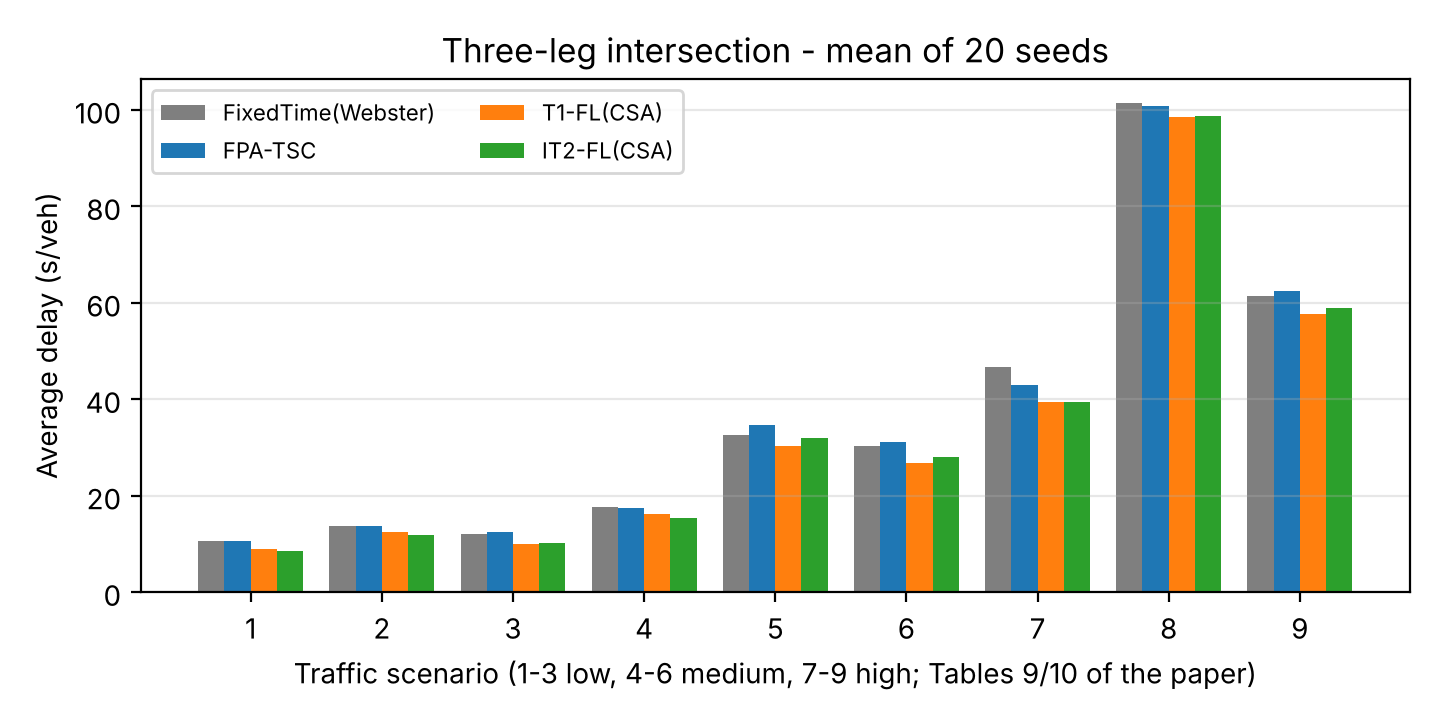
\includegraphics[width=0.49\linewidth]{baseline_delay_3leg.png}\hfill
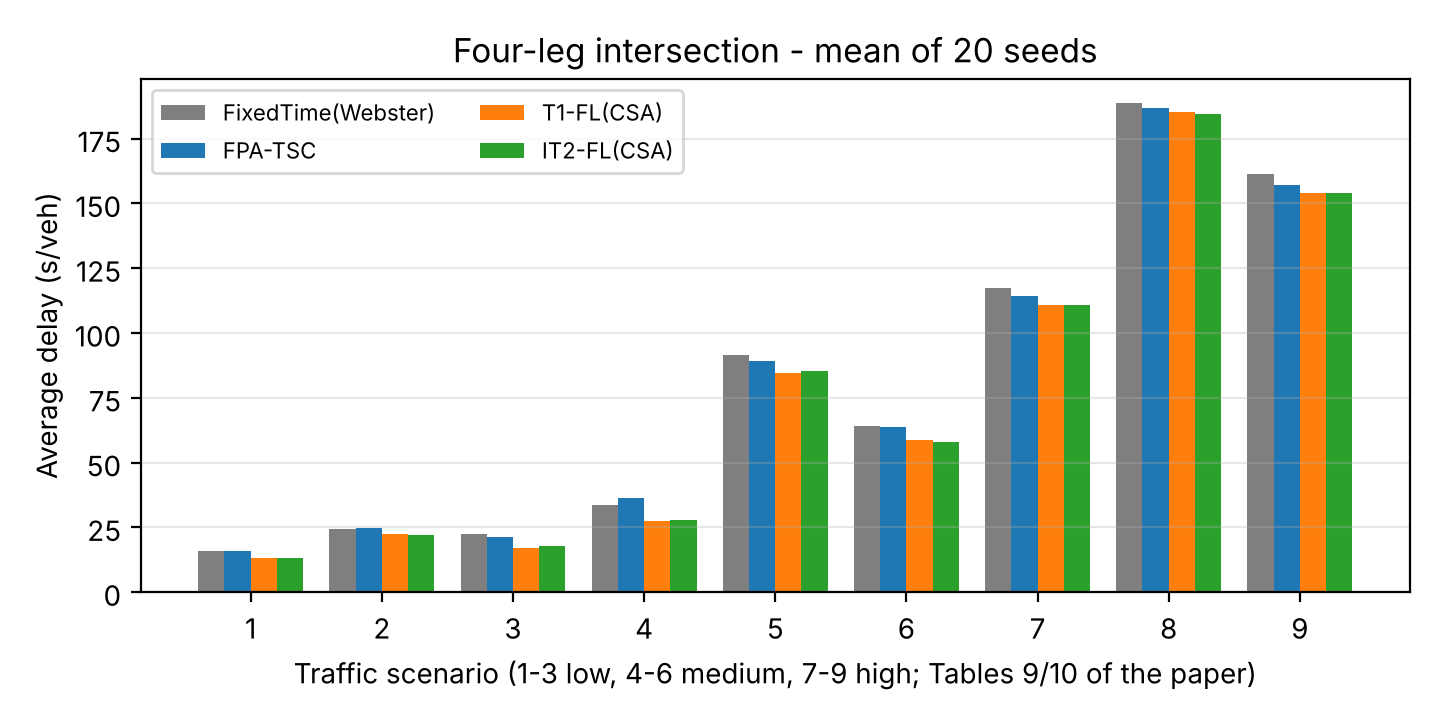
\includegraphics[width=0.49\linewidth]{baseline_delay_4leg.png}
\caption{Average delay per scenario (1--3 low, 4--6 medium, 7--9 high demand): 3-leg (left), 4-leg (right).}\label{fig:delay3}\label{fig:delay4}
\end{figure}

Per scenario, paired Wilcoxon tests (20 seeds, unadjusted) give mixed signs for IT2 versus T1: IT2 is better in 3-leg low\_equal400 ($+6.0\%$, $p=0.009$), 4-leg med\_mixed ($+1.2\%$, $p=0.036$) and 4-leg high\_equal1200 ($+0.4\%$, $p=0.011$), whereas T1 is better in 3-leg med\_equal800 ($-5.7\%$, $p=0.002$), med\_mixed ($-4.3\%$, $p=0.006$) and high\_mixed ($-2.4\%$, $p=0.004$); the other 12 scenarios show no significant difference (\texttt{baseline\_wilcoxon.csv}).

\subsection{Extension A: which optimiser?}
With 1\,220 evaluations per run and three runs per scenario, the mean test-delay reduction relative to the uniform-MF IT2 system is 12.3\% (CSA), 11.5\% (FPA), 11.2\% (PSO) and 12.4\% (DE) (Table~\ref{tab:opt}, Fig.~\ref{fig:opt}). The Friedman test over the 18 scenarios is significant ($\chi^2=33.0$, $p=3\cdot10^{-7}$); CSA is better than FPA ($p=0.002$) and PSO ($p<0.001$, Holm-adjusted Wilcoxon) but not distinguishable from DE ($p=0.30$), which has the best mean rank. The run-to-run standard deviation of the mean gain is only 0.1--0.3 percentage points, so the ranking is stable.

\begin{table}[t]
\centering\small
\caption{Optimiser comparison for the IT2 controller (18 scenarios $\times$ 3 runs, 20 test seeds). $p$: Holm-adjusted Wilcoxon test of CSA against the method.}\label{tab:opt}
\begin{tabular}{@{}lrrrrr@{}}
\toprule
Optimiser & gain vs.\ uniform MF (\%) & std over runs (pp) & mean test delay (s) & mean rank & $p$ vs CSA \\ \midrule
CSA & 12.35 & 0.30 & 54.22 & 1.83 & -- \\
FPA & 11.52 & 0.19 & 54.51 & 3.28 & 0.002 \\
PSO & 11.23 & 0.13 & 54.60 & 3.44 & $<0.001$ \\
DE & 12.44 & 0.17 & 54.16 & 1.44 & 0.30 \\ \bottomrule
\end{tabular}
\end{table}

\begin{figure}[t]
\centering
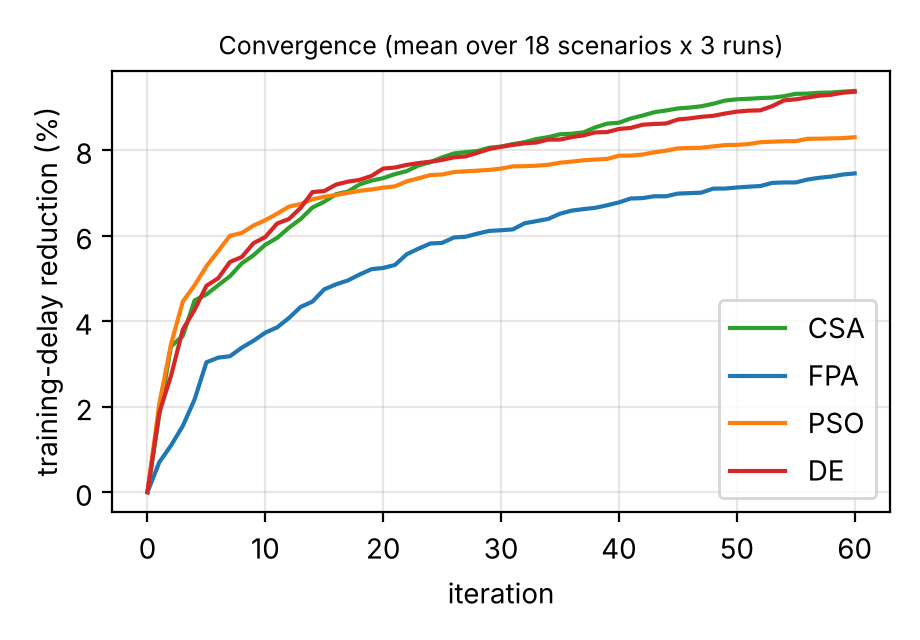
\includegraphics[width=0.49\linewidth]{optimizer_convergence.png}\hfill
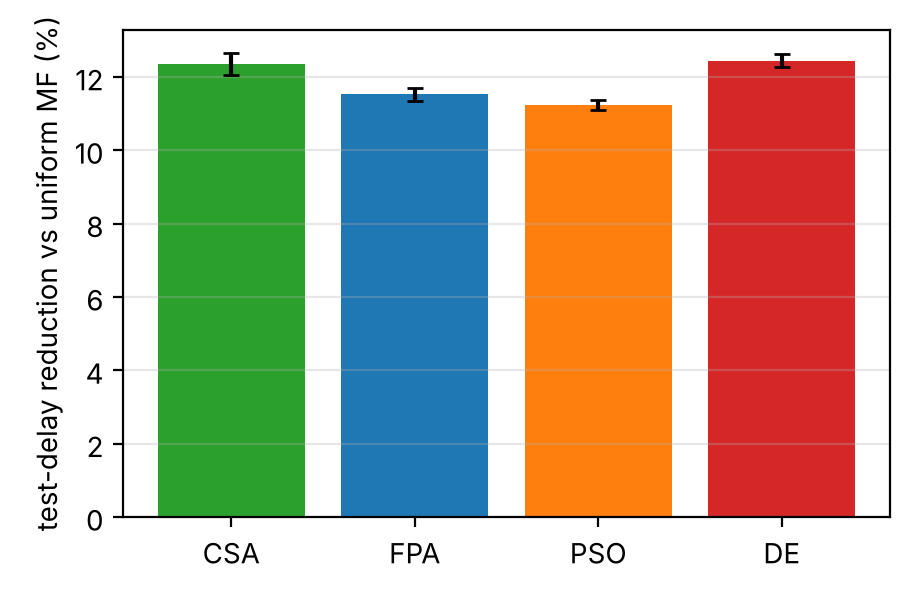
\includegraphics[width=0.49\linewidth]{optimizer_gain.png}
\caption{Convergence on the training seeds (left) and test-delay reduction with run-to-run standard deviation (right).}\label{fig:opt}
\end{figure}

\subsection{Extension B: detector noise}
Table~\ref{tab:noise} and Fig.~\ref{fig:noise} show the gain over fixed time when both inputs are disturbed by multiplicative Gaussian noise (MFs tuned noise-free). Both controllers lose benefit steadily, from about 10\% without noise to about 4\% at $\sigma=75\%$, but they never become worse than fixed time. IT2 loses slightly less than T1 at $\sigma\ge30\%$ (delay increase of 4.5\% vs.\ 5.4\% at $\sigma=50\%$ and 6.9\% vs.\ 7.8\% at 75\%), but over the 18 scenarios the difference is not significant at any noise level (Wilcoxon $p=0.44$--$1.0$). Hypothesis $H_1$ is therefore \emph{not confirmed}: the direction agrees with the Type-2 argument, the evidence does not.

\begin{table}[t]
\centering\small
\caption{Detector-noise study (mean over 18 scenarios). Gain = delay reduction versus fixed FPA-TSC; increase = delay increase relative to the noise-free controller.}\label{tab:noise}
\begin{tabular}{@{}rrrrrr@{}}
\toprule
$\sigma$ (\%) & T1 gain (\%) & IT2 gain (\%) & T1 increase (\%) & IT2 increase (\%) & $p$ \\ \midrule
0 & 10.35 & 10.17 & 0.00 & 0.00 & 0.80 \\
10 & 9.59 & 9.60 & 0.93 & 0.66 & 0.83 \\
20 & 9.08 & 9.08 & 1.48 & 1.30 & 0.87 \\
30 & 7.74 & 8.02 & 3.05 & 2.53 & 1.00 \\
50 & 5.69 & 6.29 & 5.40 & 4.53 & 0.44 \\
75 & 3.66 & 4.24 & 7.75 & 6.90 & 0.80 \\ \bottomrule
\end{tabular}
\end{table}

\begin{figure}[t]
\centering
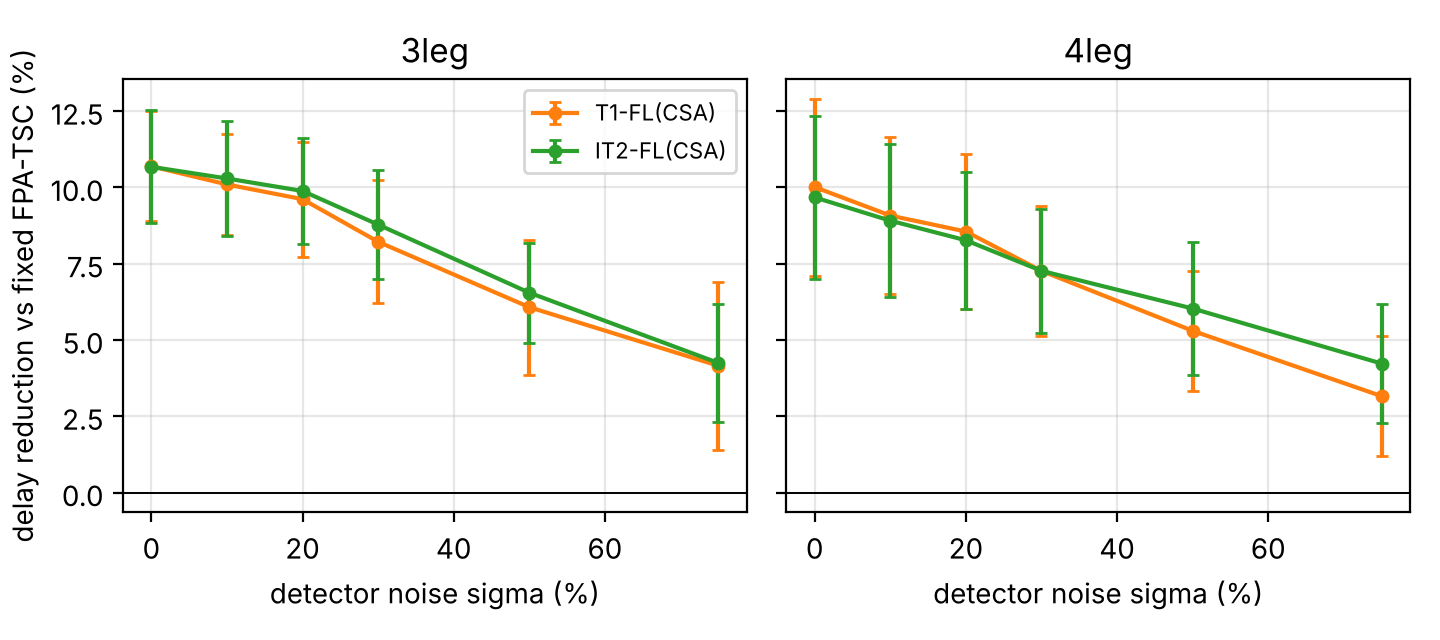
\includegraphics[width=0.78\linewidth]{noise_robustness.png}
\caption{Delay reduction versus fixed time as a function of detector noise (error bars: standard error over 9 scenarios).}\label{fig:noise}
\end{figure}

\subsection{Extension C: type reduction, cost and search budget}
With the same tuned MFs, Nie--Tan gives a slightly higher mean delay than Karnik--Mendel (54.62 vs.\ 54.28~s, $+0.6\%$, Wilcoxon $p=10^{-4}$ over 360 paired runs); note that the MFs were tuned with KM, which favours KM. Nie--Tan is cheaper (Table~\ref{tab:cost}). Increasing the CSA budget from 100 to 400 iterations lowered the \emph{training} delay but not reliably the test delay: of eight cases, the test delay improved in two (IT2: 3-leg med\_equal800 31.9$\to$30.5~s and high\_mixed 59.0$\to$57.4~s) and became worse in six (\texttt{budget\_study\_summary.csv}). Tuning on only four seeds therefore over-fits, and the larger IT2 parameter space did not simply need more search.

\begin{table}[t]
\centering\small
\caption{Computational cost on 2 vCPU (median of 5 repeats).}\label{tab:cost}
\begin{tabular}{@{}lrr@{}}
\toprule
System & inference per decision ($\mu$s) & one 900~s simulation (ms) \\ \midrule
Fixed time & -- & 0.23 \\
Type-1 Sugeno & 14.5 & 0.75 \\
IT2 Sugeno, Nie--Tan & 34.7 & 1.45 \\
IT2 Sugeno, Karnik--Mendel & 51.3 & 2.19 \\ \bottomrule
\end{tabular}
\end{table}

\section{Discussion}
\textbf{Agreement with the paper.} Qualitatively the paper's first conclusion holds: scenario-tuned fuzzy controllers beat fixed time (about 10\% here; 8.6--31\% in the paper). Our gain is at the lower end because our fixed-time baseline is strong: Webster and FPA greens are close to optimal for the known mean demand, so the fuzzy controller can only exploit random fluctuations of the arrivals. The paper does not state how its fixed-time plan was set.

\textbf{Disagreement.} The advantage of Type-2 over Type-1 (2.4--5.7\% in the paper) was not reproduced: the two systems are equal on average and differ in sign across scenarios. Plausible causes, which this study cannot separate completely: (i) in the paper the Type-1 competitor differs in optimiser and phase optimisation, so part of its 2.4--5.7\% may not be due to the fuzzy type; (ii) our simulation is noise-free apart from random arrivals, so a footprint of uncertainty has little to absorb, and even with added detector noise the benefit of IT2 is at most 1 percentage point and not significant; (iii) our rule table is monotone and fixed, so tuning the MFs is the only degree of freedom, and 65 parameters tuned on four seeds are prone to over-fitting (Section~\ref{sec:results}, Extension C); (iv) our single-intersection model with split phasing differs from KU-Trsim.

\textbf{What explains the gain.} Uniform MFs give no benefit, so the controller works because CSA moves the MFs to the demand level: it learns a scenario-specific mapping from (vehicles, queue) to a green change, which acts like a feedback correction of the cycle. This is also why the controller is tuned per scenario, as in the paper, and why in practice the demand level would first have to be recognised.

\textbf{Optimisers.} CSA, the paper's choice, is competitive: it is significantly better than FPA and PSO but equal to DE at equal budget, so there is no evidence that CSA is special. Run time per tuning (about 21~s) was the same for all four because the simulation dominates the cost.

\textbf{Cost.} IT2 inference costs 3.5 times (KM) or 2.4 times (Nie--Tan) the Type-1 inference, which is negligible for a decision taken once per phase, but IT2 tuning is about 3 times slower than Type-1 tuning in our runs (73--174~s vs.\ 25--53~s for 400 iterations). Nie--Tan costs 0.6\% more delay for a one-third cheaper inference, a reasonable trade for embedded use.

\section{Limitations}
\begin{itemize}\setlength\itemsep{0pt}
\item \textbf{Simulator.} The mesoscopic simulator has no car following, no turning movements, no acceleration tables and a single 15-min run per seed. Absolute delays cannot be compared with the paper; only the direction and relative size of the effects can.
\item \textbf{Phase plan.} Split phasing (one phase per leg) is used for all scenarios. With four legs and 900--1200 veh/h per leg this saturates the intersection ($X>1$), so all controllers are close to each other and delays (111--187~s) are far above those of the paper (about 75--81~s); the paper presumably used phase plans with several approaches per phase. The 4-leg high-demand results should be read as an over-saturation study. FPA phase-plan selection, phase-order optimisation every three cycles and the left-turn-pocket geometries were not reproduced.
\item \textbf{Unpublished details} (rule table, lower-MF height, population sizes, headway factors) were assumed (Table~\ref{tab:diff}); a different rule table could change the Type-1/Type-2 comparison.
\item \textbf{Tuning protocol.} Four training seeds, one demand level per tuning, and 20--33 times fewer iterations than the paper's 2000; the test seeds are disjoint, which makes the comparison fair but also exposes the over-fitting.
\item \textbf{Statistics.} The nine scenarios per geometry are not random samples, per-scenario Wilcoxon $p$-values are not corrected for multiple testing, and noise was modelled only as multiplicative Gaussian error on both inputs.
\item \textbf{Bibliography.} Seven classic references were cited from memory and not re-checked online (see \texttt{references/}\allowbreak\texttt{README.md}).
\end{itemize}

\section{Conclusion}
We re-implemented the fuzzy green-time part of a hybrid FPA/CSA/Type-2 traffic controller in an own simulator and re-ran its main experiment on 18 scenarios. Tuned Type-1 and interval Type-2 Sugeno controllers lowered delay by about 10\% against well-set fixed-time control, confirming the main claim in direction, but the additional benefit of Type-2 reported by the paper (2.4--5.7\%) did not appear. The extensions show that (a) CSA performs on par with DE and better than FPA and PSO at equal budget, (b) both controllers keep a positive benefit up to 75\% detector noise and IT2 degrades slightly less, though not significantly, (c) Nie--Tan type reduction is a cheap substitute for Karnik--Mendel at 0.6\% extra delay, and (d) more tuning iterations over-fit to the training seeds. Future work: phase-plan selection with several approaches per phase and left-turn movements, tuning with more seeds or a robust objective, learning the rule base, and noise models closer to real detectors.

\section*{Generative AI Usage Disclosure}
A generative AI assistant (Claude, Anthropic; used through the Claude app / Claude Code in November 2026) was used extensively in this project.
\textbf{Code development:} the simulator, the fuzzy controllers, the four optimisers and the experiment and analysis scripts (\texttt{src/}, \texttt{experiments/}) were drafted by the assistant and then checked with
unit tests (Karnik--Mendel against brute-force enumeration, Type-2 $\to$ Type-1 limit, rule-table monotonicity), by comparing the simulator with the HCM delay model, and by re-running the complete baseline experiment, which reproduced the stored results.
\textbf{Debugging} and \textbf{concept explanation} (Type-2 sets, type reduction, the metaheuristics) were done with the assistant.
\textbf{Literature search:} the assistant proposed related work. Entries copied from the reference list of the reference paper are cited only for what that paper reports about them;
the other recent studies (Koukol, Agrahari, Bi 2024, Li \emph{et al.}) were looked up online and their bibliographic data were read from the publisher pages; textbook classics were cited from memory and are flagged in \texttt{references/README.md}.
No reference was kept that could not be traced to one of these sources.
\textbf{Writing:} the assistant drafted the report, the slides and the README, and edited the language.
\textbf{Results:} every number in this report is produced by the code in the repository (result files in \texttt{results/}); no result of the reference paper was reused as our own, and the paper's numbers appear only in
comparison columns that are labelled as such. The code of the reference paper's authors was not used (none is public).
\emph{[Student: replace this sentence by a statement of your own about which parts you ran, read and can explain, as required by Section~15 of the project guideline.]}

% IEEE-style reference list (hand-formatted because IEEEtran.cls is not installed in the build environment).
% Verification status of every entry is documented in references/README.md.
\begin{thebibliography}{99}\small\raggedright\sloppy

\bibitem{ref_paper} E. Korkmaz and A. P. Akg{\"u}ng{\"o}r, ``A hybrid traffic controller system based on flower pollination algorithm and type-2 fuzzy logic optimized with crow search algorithm for signalized intersections,'' \emph{Soft Comput.}, vol. 28, pp. 7227--7249, 2024, doi: 10.1007/s00500-024-09643-w.

\bibitem{korkmaz2021a} E. Korkmaz and A. P. Akg{\"u}ng{\"o}r, ``Optimizing of phase plan, sequence and signal timing based on flower pollination algorithm for signalized intersections,'' \emph{Soft Comput.}, vol. 25, pp. 4243--4259, 2021.

\bibitem{dogan2016} E. Do{\u g}an and A. P. Akg{\"u}ng{\"o}r, ``Optimizing a fuzzy logic traffic signal controller via the differential evolution algorithm under different traffic scenarios,'' \emph{Simulation}, vol. 92, pp. 1013--1023, 2016.

\bibitem{trabia1999} M. B. Trabia, M. S. Kaseko, and M. Ande, ``A two-stage fuzzy logic controller for traffic signals,'' \emph{Transp. Res. C, Emerg. Technol.}, vol. 7, pp. 353--367, 1999.

\bibitem{chen2006} J. Chen and L. Xu, ``Road-junction traffic signal timing optimization by an adaptive particle swarm algorithm,'' in \emph{Proc. 9th Int. Conf. Control, Autom., Robot. Vis. (ICARCV)}, 2006, pp. 1--7.

\bibitem{balaji2009} P. G. Balaji and D. Srinivasan, ``Distributed multi-agent type-2 fuzzy architecture for urban traffic signal control,'' in \emph{Proc. IEEE Int. Conf. Fuzzy Syst.}, 2009, pp. 1627--1632.

\bibitem{bi2014} Y. Bi, D. Srinivasan, X. Lu \emph{et al.}, ``Type-2 fuzzy multi-intersection traffic signal control with differential evolution optimization,'' \emph{Expert Syst. Appl.}, vol. 41, pp. 7338--7349, 2014.

\bibitem{araghi2017} S. Araghi, A. Khosravi, D. Creighton, and S. Nahavandi, ``Influence of meta-heuristic optimization on the performance of adaptive interval type2-fuzzy traffic signal controllers,'' \emph{Expert Syst. Appl.}, vol. 71, pp. 493--503, 2017.

\bibitem{khooban2017} M. H. Khooban, N. Vafamand, A. Liaghat, and T. Dragicevic, ``An optimal general type-2 fuzzy controller for urban traffic network,'' \emph{ISA Trans.}, vol. 66, pp. 335--343, 2017.

\bibitem{lin2022} H. Lin, Y. Han, W. Cai, and B. Jin, ``Traffic signal optimization based on fuzzy control and differential evolution algorithm,'' \emph{IEEE Trans. Intell. Transp. Syst.}, 2022.

\bibitem{islam2022} Z. Islam, M. Abdel-Aty, and M. Mahmoud, ``Using CNN-LSTM to predict signal phasing and timing aided by high-resolution detector data,'' \emph{Transp. Res. C, Emerg. Technol.}, vol. 141, Art. no. 103742, 2022.

\bibitem{zhao2022} W. Zhao, Y. Ye, J. Ding \emph{et al.}, ``IPDALight: Intensity- and phase duration-aware traffic signal control based on reinforcement learning,'' \emph{J. Syst. Archit.}, vol. 123, Art. no. 102374, 2022.

\bibitem{koukol2015} M. Koukol, L. Zaj{\'i}{\v c}kov{\'a}, L. Marek, and P. Tu{\v c}ek, ``Fuzzy logic in traffic engineering: A review on signal control,'' \emph{Math. Probl. Eng.}, vol. 2015, Art. no. 979160, 2015, doi: 10.1155/2015/979160.

\bibitem{agrahari2024} A. Agrahari, M. M. Dhabu, P. S. Deshpande, A. Tiwari, M. A. Baig, and A. D. Sawarkar, ``Artificial intelligence-based adaptive traffic signal control system: A comprehensive review,'' \emph{Electronics}, vol. 13, no. 19, Art. no. 3875, 2024, doi: 10.3390/electronics13193875.

\bibitem{bi2024} Y. Bi, Q. Ding, Y. Du, D. Liu, and S. Ren, ``Intelligent traffic control decision-making based on type-2 fuzzy and reinforcement learning,'' \emph{Electronics}, vol. 13, no. 19, Art. no. 3894, 2024, doi: 10.3390/electronics13193894.

\bibitem{zadeh1965} L. A. Zadeh, ``Fuzzy sets,'' \emph{Inf. Control}, vol. 8, no. 3, pp. 338--353, 1965.

\bibitem{zadeh1975} L. A. Zadeh, ``The concept of a linguistic variable and its application to approximate reasoning---I,'' \emph{Inf. Sci.}, vol. 8, pp. 199--249, 1975.

\bibitem{takagi1985} T. Takagi and M. Sugeno, ``Fuzzy identification of systems and its applications to modeling and control,'' \emph{IEEE Trans. Syst., Man, Cybern.}, vol. SMC-15, no. 1, pp. 116--132, 1985.

\bibitem{liang2000} Q. Liang and J. M. Mendel, ``Interval type-2 fuzzy logic systems: Theory and design,'' \emph{IEEE Trans. Fuzzy Syst.}, vol. 8, pp. 535--550, 2000.

\bibitem{karnik2001} N. N. Karnik and J. M. Mendel, ``Centroid of a type-2 fuzzy set,'' \emph{Inf. Sci.}, vol. 132, no. 1--4, pp. 195--220, 2001.

\bibitem{mendel2017} J. M. Mendel, \emph{Uncertain Rule-Based Fuzzy Systems: Introduction and New Directions}, 2nd ed. Cham, Switzerland: Springer, 2017.

\bibitem{li2018nt} J. Li, R. John, S. Coupland, and G. Kendall, ``On Nie--Tan operator and type-reduction of interval type-2 fuzzy sets,'' \emph{IEEE Trans. Fuzzy Syst.}, vol. 26, no. 2, pp. 1036--1039, 2018, doi: 10.1109/TFUZZ.2017.2666842.

\bibitem{askarzadeh2016} A. Askarzadeh, ``A novel metaheuristic method for solving constrained engineering optimization problems: Crow search algorithm,'' \emph{Comput. Struct.}, vol. 169, pp. 1--12, 2016.

\bibitem{yang2012} X.-S. Yang, ``Flower pollination algorithm for global optimization,'' in \emph{Unconventional Computation and Natural Computation}. Berlin, Germany: Springer, 2012, pp. 240--249.

\bibitem{mantegna1994} R. N. Mantegna, ``Fast, accurate algorithm for numerical simulation of L{\'e}vy stable stochastic processes,'' \emph{Phys. Rev. E}, vol. 49, no. 5, pp. 4677--4683, 1994.

\bibitem{kennedy1995} J. Kennedy and R. Eberhart, ``Particle swarm optimization,'' in \emph{Proc. IEEE Int. Conf. Neural Netw.}, vol. 4, 1995, pp. 1942--1948.

\bibitem{storn1997} R. Storn and K. Price, ``Differential evolution---A simple and efficient heuristic for global optimization over continuous spaces,'' \emph{J. Global Optim.}, vol. 11, no. 4, pp. 341--359, 1997.

\bibitem{webster1958} F. V. Webster, ``Traffic signal settings,'' Road Research Technical Paper No.~39, Her Majesty's Stationery Office, London, U.K., 1958.

\bibitem{hcm2000} Transportation Research Board, \emph{Highway Capacity Manual 2000}. Washington, DC, USA: National Research Council, 2000.

\end{thebibliography}


\end{document}
